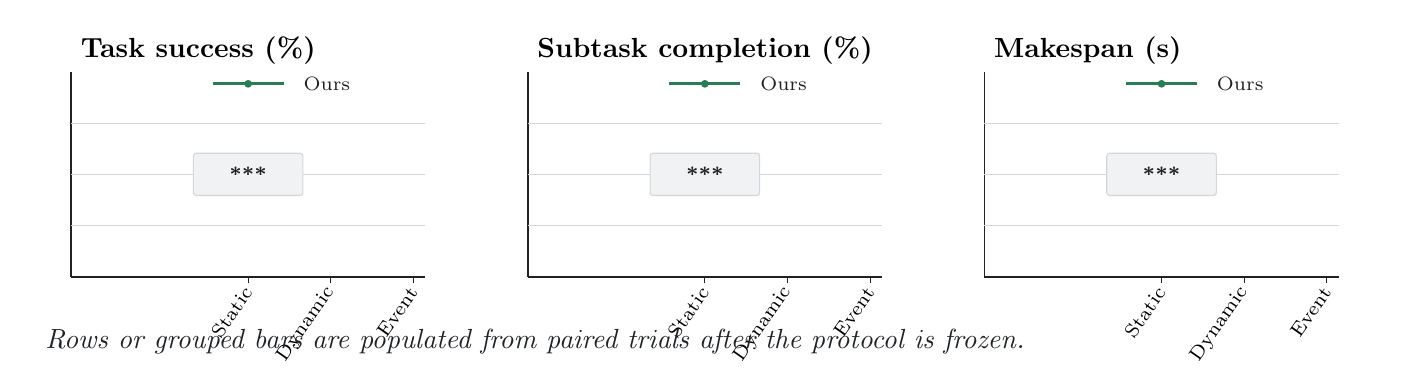
\begin{tikzpicture}[x=1cm,y=1cm,font=\rmfamily\fontsize{7.5}{8.3}\selectfont]
  \definecolor{grid}{HTML}{D4D7DA}
  \definecolor{ink}{HTML}{202326}
  \definecolor{ours}{HTML}{287D55}
  \definecolor{placeholder}{HTML}{F1F2F3}
  \foreach \x/\paneltitle in {
    0/{Task success (\%)},5.8/{Subtask completion (\%)},11.6/{Makespan (s)}}{
    \begin{scope}[shift={(\x,0)}]
      \draw[ink,line width=0.6pt] (0.55,0.55) -- (5.05,0.55);
      \draw[ink,line width=0.6pt] (0.55,0.55) -- (0.55,3.15);
      \foreach \yy in {1.20,1.85,2.50}{\draw[grid,line width=0.35pt] (0.55,\yy)--(5.05,\yy);}
      \node[anchor=west,font=\bfseries] at (0.55,3.42) {\paneltitle};
      \foreach \xx/\lab in {2.80/{Static},3.85/{Dynamic},4.90/{Event}}{
        \draw[ink,line width=0.35pt] (\xx,0.55)--(\xx,0.47);
        \node[rotate=55,anchor=east,inner sep=0pt] at (\xx,0.40) {\lab};
      }
      \node[draw=grid,fill=placeholder,rounded corners=1pt,text=ink,
            inner xsep=13pt,inner ysep=5pt] at (2.80,1.85) {\bfseries ***};
      \draw[ours,line width=1.0pt] (2.35,3.00)--(3.25,3.00);
      \fill[ours] (2.80,3.00) circle (1.4pt);
      \node[anchor=west,text=ink] at (3.38,3.00) {Ours};
    \end{scope}
  }
  \node[anchor=west,text=ink,font=\itshape] at (0.10,-0.28)
    {Rows or grouped bars are populated from paired trials after the protocol is frozen.};
  \path[use as bounding box] (0.0,-0.48) rectangle (17.15,3.65);
\end{tikzpicture}
